% Created 2022-12-15 gio 22:17
% Intended LaTeX compiler: lualatex
\documentclass[letterpaper, 11pt]{article}

\usepackage{lmodern} % Ensures we have the right font
\usepackage[T1]{fontenc} % Basic font & characters selection
\usepackage[utf8]{inputenc}
\usepackage{fontspec}
% Define font family to use (Other options are: Iosevka, Source Code Pro, Ubuntu, Titillium -> see setup file)
\setmainfont{RobotoCondensed}[Extension=.ttf, UprightFont=*-Light, BoldFont=*-Regular, ItalicFont=*-LightItalic, BoldItalicFont=*-BoldItalic, Path=/home/valentino/Dropbox/fonts/]

% Tables, wrapping, and other options
%\usepackage{longtable} % This package defines the longtable environment, a multi-page version of tabular
% For a long time, the tabular environment was used to build tables.
% However, writing tables with tabular can be troublesome for beginners and really complex tables can be near impossible to write
% Also, tables built with the tabular environment have some typographical issues and, when color is used, can be misread by PDF readers.
% Therefore, more and more LaTeX users are calling to use the tblr environment from the tabularray package instead.
% Guide at https://www.latex-tables.com/ressources/tabularray.html (To merge cells cell{5}{1} = {c=2}{})
\usepackage{tabularray} % In order to get tblr env
\usepackage{wrapfig} % This makes the wrapfigure environment available
\usepackage{rotating} % Pretty obvious
\usepackage[normalem]{ulem} % underlining and strike-through
\usepackage{capt-of} % Captions outside of floats
\usepackage{graphicx} % Include images
\usepackage{amsmath, amsthm, amssymb, mathtools} % Subscript & superscript and math environments (amsmath),  Various symbols used for interpreting the entities (amssymb)
%% Memo for table setup
%% h -> Place the float here, i.e., approximately at the same point it occurs in the source text (however, not exactly at the spot)
%% t -> Position at the top of the page
%% b -> Position at the bottom of the page
%% p -> Put on a special page for floats only
%% ! -> Override internal parameters LaTeX uses for determining "good" float positions
%% H -> Places the float at precisely the location in the LaTeX code (Requires the float package)
\usepackage[table, xcdraw]{xcolor}
\usepackage{float} % Needed for table[H] override
\usepackage{listings} % Code highlighting
\usepackage{mdframed} % \usepackage[framemethod=TikZ]{mdframed} (Alternativa in caso si voglia usare Tikz come metodo)

% COLOR DEFINITION
\definecolor{classTIKZcolor}{RGB}{222,222,222}
% DEFINIZIONE COLORI TIKZ
\definecolor{darkblue}{RGB}{0,60,104}
\definecolor{darkdark}{RGB}{22,22,22}
% DEFINIZIONE COLORI DA USARE PER IL CODICE
\definecolor{airforceblue}{rgb}{0.36, 0.54, 0.66}

% Definizione colori per i linguaggi da usare
\definecolor{orangered}{RGB}{239,134,64}
\definecolor{includeStatementCPP}{RGB}{148,123,155}
\definecolor{libraryStatementCPP}{RGB}{126,190,184}
\definecolor{colorMainCPP}{RGB}{190,116,67}
\definecolor{colorTypesCPP}{RGB}{188,90,69}
\definecolor{colorReservedKeywordsCPP}{RGB}{130,183,75}
\definecolor{colorLoopsCPP}{RGB}{185,176,176}
\definecolor{colorOtherKeywordsCPP}{RGB}{254,178,54}
\definecolor{headerJava}{HTML}{006b3C}
\definecolor{packageNameJavaDefinition}{HTML}{007BA7}
\definecolor{classKeywordJava}{HTML}{CD5C5C}
\definecolor{classNameJava}{HTML}{D2691E}
\definecolor{methodKeyword}{HTML}{FE6F5E}
\definecolor{constantsKeyword}{HTML}{FFA812}
\definecolor{attributesKeyword}{HTML}{9955BB}
\definecolor{testKeyword}{HTML}{1E90FF}
\definecolor{assertKeyword}{HTML}{6082B6}
\definecolor{expectedKeyword}{HTML}{29AB87}
\definecolor{nullKeyword}{HTML}{E66771}
\definecolor{variableKeyword}{HTML}{778899}
% Definizione colori definitiva
\definecolor{orangelight}{RGB}{238,162,82}
\definecolor{orange-apricot}{HTML}{FBCEB1}
\definecolor{greenlight}{RGB}{147,196,125}
\definecolor{purplelight}{RGB}{176,159,222}
\definecolor{bluelight}{RGB}{122,171,216}
\definecolor{lavanda}{HTML}{F4BBFF}

% Definizione gradiente di colori
% Azure
\definecolor{customAzure1}{HTML}{B1E7E1}
\definecolor{customAzure2}{HTML}{A1E2DB}
\definecolor{customAzure3}{HTML}{92DDD6}
\definecolor{customAzure4}{HTML}{83D8CF}
\definecolor{customAzure5}{HTML}{73D3C9}
\definecolor{customAzure6}{HTML}{64CEC3}
\definecolor{redstrong}{RGB}{255,40,50}
\definecolor{greendark}{RGB}{144,161,106}
\definecolor{footerColor}{RGB}{0,163,243}
\definecolor{footerColorSurrounding}{RGB}{22,154,255}
\definecolor{ygroblue}{HTML}{179AFF}
% TIKZ
\usepackage{tikz}
% DEFINIZIONE CAMPI E FORME PER TIKZ
\usetikzlibrary{calc,shadows,shapes,arrows,backgrounds,graphdrawing.trees, decorations.pathreplacing,positioning, arrows.meta}

% DEFINIZIONE FORME GEOMETRICHE PER DIAGRAMMI
\tikzstyle{CIRCLE} = [circle, minimum width=0.8cm, minimum height=0.8cm,text centered, draw=black, fill=blue!30]
\tikzstyle{CIRCLESMALL} = [circle, minimum width=0.2cm, minimum height=0.2cm,text centered, draw=black, fill=black]
\tikzstyle{startstop} = [rectangle, rounded corners, minimum width=3cm, minimum height=1cm,text centered, draw=black, fill=red!30]
\tikzstyle{io} = [trapezium, trapezium left angle=70, trapezium right angle=110, minimum width=3cm, minimum height=1cm, text centered, draw=black, fill=blue!30]
\tikzstyle{process} = [rectangle, minimum width=3cm, minimum height=1cm, text centered, text width=3cm, draw=black, fill=orange!30]
\tikzstyle{decision} = [diamond, minimum width=3cm, minimum height=1cm, text centered, draw=black, fill=green!30]
\tikzstyle{class}=[rectangle, draw=black, text centered, anchor=north, text=black, text width=3cm, shading=axis, bottom color=classTIKZcolor,top color=white,shading angle=45]
\tikzstyle{arrow} = [thick,->,>=stealth]
% Tree forest
\usepackage[linguistics]{forest} %\usepackage{forest}


% OPTIONS FOR MDFRAMES (ENVIRONMENT)
\makeatletter
\mdfdefinestyle{@mdf@stubenv}{
leftmargin=2pt,
rightmargin=2pt,
innermargin=0pt,
outermargin=0pt,
skipabove=2pt,
skipbelow=2pt,
linewidth=1pt,
linecolor=stub@tmp!80!black,
frametitlebackgroundcolor=stub@tmp!80!black,
backgroundcolor=stub@tmp,
innertopmargin=1pt,
innerbottommargin=1pt,
innerleftmargin=1pt,
innerrightmargin=1pt,
nobreak=true}
\def\make@stubenv#1#2#3#4{
\global\newcounter{stub@#1}[#4]
\newenvironment{#1}[1][]{
\colorlet{stub@tmp}{#2!25}
\begin{mdframed}[style=@mdf@stubenv, frametitle={\scriptsize \% #3 ##1}]
}{
\global\stepcounter{stub@#1}\end{mdframed}
}
}
\make@stubenv{definition}{ygroblue}{}{subsection}
\makeatother

% SET DEFAULT OPTION FOR CODE BLOCKS
\lstset {
frame=trBL, %frame=single
framesep=\fboxsep,
framerule=\fboxrule,
frameround=fttt,
rulecolor=\color{black},
xleftmargin=\dimexpr\fboxsep+\fboxrule,
xrightmargin=\dimexpr\fboxsep+\fboxrule,
breaklines=true,
basicstyle=\small\tt,
keywordstyle=\color{blue}\sf,
columns=flexible,
}

% Settaggio stile per i linguaggi da usare
\lstdefinestyle{CPP}{
language=C++,
backgroundcolor=\color{white},
escapeinside={`'},
numbers=left,
numbersep=15pt,
numberstyle=\tiny,
commentstyle=\color{gray},
% #include statement
keywords=[1]{\#include},
keywords=[2]{ main },
% types
keywords=[3]{int, char, short, long, float, double},
% List of reserved keywords
keywords=[4]{auto, struct , unsigned, signed, enum, register, typedef, extern, return, union, continue, goto, volatile, default, define, static},
% Loops
keywords=[5]{do, while, case, else, switch, break, for, if},
% List of other keywords
keywords=[6]{void, boolean, const, sizeof, sleep},
% Colors of the keywords:
keywordstyle=[1]\color{includeStatementCPP},
keywordstyle=[2]\color{colorMainCPP},
keywordstyle=[3]\color{colorTypesCPP},
keywordstyle=[4]\color{colorReservedKeywordsCPP},
keywordstyle=[6]\color{colorOtherKeywordsCPP}
}
\lstdefinestyle{BASH}{
language=bash,
commentstyle=\color{gray},
backgroundcolor=\color{white},
numbers=left,
numbersep=15pt,
numberstyle=\tiny,
stringstyle=\color{greendark},
commentstyle=\color{gray},
keywords=[1]{exit, print_error, fail},
keywords=[2]{printf, cut, print_ok, basename, while, usage, run},
keywords=[3]{ls, find, touch, egrep, print_info, read, done},
keywords=[4]{wc},
keywordstyle=[1]\color{redstrong},
keywordstyle=[2]\color{greenlight},
keywordstyle=[3]\color{bluelight},
keywordstyle=[4]\color{purplelight}
}
\lstdefinestyle{JAVA}{
language=Java,
backgroundcolor=\color{white},
numbers=left,
numbersep=15pt,
numberstyle=\tiny,
commentstyle=\color{gray},
stringstyle=\color{gray},
keywords=[1]{package, import, static, public, return, true},
keywords=[2]{android, Manifest, content, Context, util, Log, androidx, core, app, ActivityCompat, org, test, platform, app, InstrumentationRegistry, ext, junit, runner, runners, AndroidJUnit4, Test, RunWith, Assert, com, natour, utils, constants, Constants, persistence, LocalUser, LocalUserDbManager, java, regex, Pattern, Before},
keywords=[3]{void, boolean, int, String, while, synchronized, volatile, long, double},
keywords=[4]{class, @RunWith, super},
keywords=[5]{if, Employee, try, catch},
keywords=[6]{localUser, dbManager, checkFineLocation, checkCoarseLocation, appContext, controlloRecuperoPassword},
keywords=[7]{private},
keywords=[8]{@Test, @Before},
keywords=[9]{assertTrue, assertFalse},
keywords=[10]{expected, IllegalArgumentException},
keywords=[11]{null, false},
keywords=[12]{username, email, password, confermaPassword, pattern},
keywordstyle=[1]\color{headerJava},
keywordstyle=[2]\color{packageNameJavaDefinition},
keywordstyle=[3]\color{methodKeyword},
keywordstyle=[4]\color{classKeywordJava},
keywordstyle=[5]\color{classNameJava},
keywordstyle=[6]\color{attributesKeyword},
keywordstyle=[7]\color{constantsKeyword},
keywordstyle=[8]\color{testKeyword},
keywordstyle=[9]\color{assertKeyword},
keywordstyle=[10]\color{expectedKeyword},
keywordstyle=[11]\color{nullKeyword},
keywordstyle=[12]\color{variableKeyword},
morekeywords={*,...}
}
\lstdefinestyle{XML}{
language=XML,
backgroundcolor=\color{white},
numbers=left,
numbersep=15pt,
numberstyle=\tiny,
commentstyle=\color{gray},
keywords=[1]{article, author, title, description, text, formula, math},
keywords=[2]{dbs:,dbs:book,<dbs:description>},
keywordstyle=[1]\color{colorMainCPP},
keywordstyle=[2]\color{includeStatementCPP},
}

% Colorizing links in a nicer way.
\usepackage{hyperref} % Links
\hypersetup{colorlinks, linkcolor=black, urlcolor=blue}
%\hypersetup{pdfauthor={%a}, pdftitle={%t}, pdfkeywords={%k}, pdfsubject={%d}, pdfcreator={%c}, pdflang={%L}, breaklinks=true, colorlinks=true, linkcolor=link, urlcolor=url, citecolor=cite\n}
%Bibliography (Not added yet)
\usepackage[backend=biber,sortcites,style=verbose-trad2]{biblatex}
\bibliography{./Bibliography.bib}
\usepackage{titling}
\setlength{\droptitle}{-9em}
\setlength{\parindent}{0pt}
\setlength{\parskip}{1em}
\usepackage[stretch=10]{microtype}
\usepackage{hyphenat}
\usepackage{ragged2e}
\usepackage{subfig} % Subfigures (not needed in Org I think)
\usepackage[top=1in, bottom=1.25in, left=0.55in, right=0.55in, showframe]{geometry} % Page geometry (to show frames add showframe options)
\renewcommand{\baselinestretch}{1.15}
% Page numbering - Footer
\usepackage{fancyhdr} % Custom headers and footers
\pagestyle{fancy} % Makes all pages in the document conform to the custom headers and footers
\fancyhead{} % No page header
\renewcommand{\headrulewidth}{0pt}
\fancyfoot[L]{} % Empty left footer
\fancyfoot[C]{} % Empty center footer
\newcommand\FrameBoxR[1]{
\fcolorbox{footerColorSurrounding}{footerColor}{\makebox[3cm][r]{\textcolor{white}{\bfseries#1}}}
}
\fancyfoot[R]{\FrameBoxR{\thepage}}
\usepackage[explicit]{titlesec}

% Title customization
\pretitle{\begin{center}\fontsize{20pt}{20pt}\selectfont}
\posttitle{\par\end{center}}
\preauthor{\begin{center}\vspace{-6bp}\fontsize{14pt}{14pt}\selectfont}
\postauthor{\par\end{center}\vspace{-25bp}}
\predate{\begin{center}\fontsize{12pt}{12pt}\selectfont}
\postdate{\par\end{center}\vspace{0em}}

% Section/subsection headings:
%Section
\titlespacing\section{0pt}{2pt}{2pt} % left margin, space before section header, space after section header
%Subsection
\titlespacing\subsection{0pt}{5pt}{-2pt} % left margin, space before subsection header, space after subsection header
%Subsubsection
\titlespacing\subsubsection{0pt}{5pt}{-2pt} % left margin, space before subsection header, space after subsection header

% List spacing & options
\usepackage{enumitem}
\usepackage{fdsymbol}
\setlist{itemsep=-2pt} % or \setlist{noitemsep} to leave space around whole list
\setlist[enumerate, 1]{label=\arabic*.}
\setlist[enumerate, 2]{label=\Roman*.}
\setlist[enumerate, 3]{label=\alph*.}
\setlist[itemize, 1]{label=$\smallblacktriangleright$}
\setlist[itemize, 2]{label=$\smalldiamond$}
\setlist[itemize, 3]{label=$\smallcircle$}
\author{Valentino Bocchetti}
\date{}
\title{}
\begin{document}

\thispagestyle{empty}
\newgeometry{margin=0pt}

\begin{tikzpicture}[remember picture, overlay]
  \begin{scope}

    % STRUTTURA ESTERNA (ANGOLI E COLORAZIONE)
    \node[
      isosceles triangle,
      isosceles triangle apex angle=90,
      draw,
      rotate=315,
      fill=darkblue,
      minimum size =55cm] (triangoloPrimoLivelloAngoloInferiore)
    at ($(current page.south east)$)
    {};

    \node[
      isosceles triangle,
      isosceles triangle apex angle=90,
      draw,
      rotate=315,
      fill=footerColorSurrounding,
      minimum size =50cm] (triangoloSecondoLivelloAngoloInferiore)
    at ($(current page.south east)$)
    {};

    \node[
      isosceles triangle,
      isosceles triangle apex angle=90,
      draw,
      rotate=315,
      fill=darkdark,
      minimum size =35cm] (triangoloTerzoLivelloAngoloInferiore)
    at ($(current page.south east)$)
    {};

    \node[
      isosceles triangle,
      isosceles triangle apex angle=90,
      draw,
      rotate=315,
      fill=white,
      minimum size =32cm] (triangoloQuartoLivelloAngoloInferiore)
    at ($(current page.south east)$)
    {};


    \node[
      isosceles triangle,
      isosceles triangle apex angle=90,
      draw,
      rotate=135,
      fill=white,
      minimum size =31cm] (triangoloSuperiore)
    at ($(current page.north west)$)
    {};


    % STRUTTURA DEL CERCHIO E IL SUO CONTENUTO
    \node [circle, minimum size=15cm, fill=white, draw=darkblue, line width = 7pt, xshift=11cm, yshift=1cm](centro)
    at ($(current page.west)$)
    {};

    \coordinate (logo) at (10.7,-7.5);
    \node[rectangle, inner sep = 0pt, outer sep = 0pt, minimum width = 3.5cm, minimum height = 3.5cm]
    at (logo){
\includegraphics[width=3.5cm, height=3.5cm]{./Risorse/Start-Page/FedericoII.png}};

    \node[scale=1.5] at (5.85,-10){\LARGE{StealBot}};

    \node[rectangle,
      draw,
      minimum width=4cm,
      minimum height=2mm,
      xshift= 6.42cm,
      yshift= -11cm,
      minimum height=2mm,
      fill = darkblue] (r) at (0,0) {};
 
    \node[scale=1.5] at (11,-13){\itshape{\LARGE{Università degli studi di Napoli}}};
    \node[scale=1.5] at (11,-15){\itshape{\LARGE{Federico II}}};


    %% STRUTTURA ANGOLO SINISTRO (angolo north-west)
    \node[scale=3] at (1,-1){
\includegraphics[height=10pt,width=10pt]{./Risorse/Start-Page/calendar.png}};
    \node[scale=2] at (6,-1){\itshape{\LARGE{A.A. 2022-2023}}};

    %% STRUTTURA ANGOLO DESTRO (angolo south-east) - Informazioni studenti
    %% Valentino Bocchetti
    \node[scale=3] at (12,-21){
\includegraphics[height=10pt,width=10pt]{./Risorse/Start-Page/graduated.png}};
    \node[scale=1.5] at (16.5, -21.23){\textbf{Valentino Bocchetti - N86003405}};

    %% Valentina Annunziata
    \node[scale=3] at (12,-22.8){
\includegraphics[height=10pt,width=10pt]{./Risorse/Start-Page/graduated_alt.png}};
    \node[scale=1.5] at (16.7, -22.9){\textbf{Valentina Annunziata - N86003280}};

    %% Francesco Ciccarelli
    \node[scale=3] at (12,-24.6){
\includegraphics[height=10pt,width=10pt]{./Risorse/Start-Page/graduated.png}};
    \node[scale=1.5] at (16.56, -24.7){\textbf{Francesco Ciccarelli - N86003285}};

    %% Giulia Caputo
    \node[scale=3] at (12,-26.4){
\includegraphics[height=10pt,width=10pt]{./Risorse/Start-Page/graduated_alt.png}};
    \node[scale=1.5] at (15.8, -26.5){\textbf{Giulia Caputo - N86003429}};
  \end{scope}

\end{tikzpicture}

\newpage
\restoregeometry
%\renewcommand*\contentsname{\hfill Indice \hfill}
%\tableofcontents
\pagebreak
\section{Presentazione}
\label{Presentazione progetto}
\noindent\makebox[\textwidth]{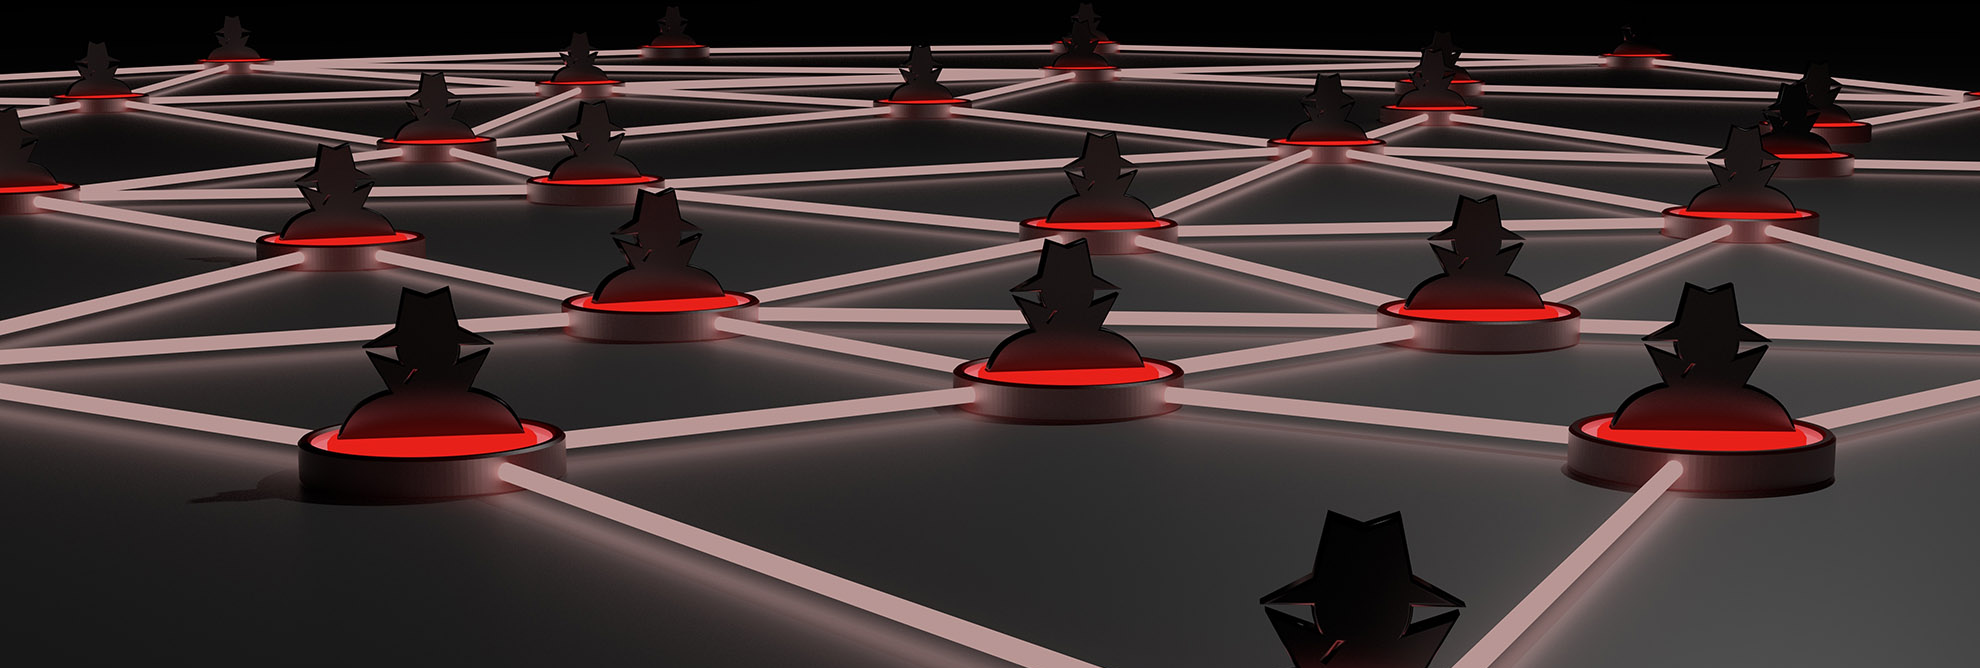
\includegraphics[width=\paperwidth]{Risorse/Title.png}}
\subsection{Descrizione della traccia}
\label{Descrizione traccia}
Si richiede la realizzazione di una \texttt{BotNET} \autocite{BOTNET} per il recupero di quante più informazioni possibili sul dispositivo in cui una delle componenti della BotNET (a scelta dello studente) venga eseguito.
\subsubsection{Tecnologie e linguaggi richiesti}
\label{Tecnologie e linguaggi}
Si richiede un applicativo scritto in \texttt{Python} \autocite{DefinizionePython} che utilizzi come strumento di comunicazione le \texttt{socket} \autocite{DefinizioneSocket}
\subsection{Implementazione del sistema}
\label{Implementazione sistema}
Il progetto si concretizza in 2 componenti ben definite:
\begin{itemize}
\item Un \texttt{Bot Master} per la gestione dei dati ricevuti dal \texttt{bot slave} al quale inpartisce comandi sfruttando una connessione tramite socket asincrona;
\item Il \texttt{Bot slave}, che ha il compito di ricavare quante più informazioni possibili sullo stato della macchina sul quale viene eseguito \autocite{notaBotSlave1} .
\end{itemize}
\vfill
\subsection{Guida al Bot Master}
\label{Guida (Bot master)}
\subsubsection{Primo avvio}
\label{Primo avvio (Bot master)}
Durante la fase di avvio il programma effettua le seguenti operazioni:
\begin{itemize}
\item Controlla che \texttt{host} e \texttt{porta} \autocite{infoHostPortMaster} siano disponibili per la successiva creazione della socket;
\item Esegue una connessione al dbms utilizzato per il salvataggio delle informazioni e inizializza la \texttt{tabella} utilizzata per lo scopo (se non precedentemente presente);
\item Inizializza la socket in attesa di nuove connessioni dal client a cui impartirà comandi da eseguire;
\end{itemize}

Nel momento in cui viene effettuata una nuova connessione, il server invia la richiesta effettuata dall'utente al client e in base a questa automaticamente:
\begin{itemize}
\item Salva l'informazione sul database (che viene mostrata all'utente attraverso lo standard output);
\item Nel caso in cui si trattasse di un file (identificato da un campo \texttt{Header} a inizio richiesta), lo salva automaticamente, per poter essere fruibile successivamente.
\end{itemize}
\subsubsection{Memorizzazione dei dati}
\label{Memorizzazione dati (Bot master)}
Il sistema permette inoltre utilizza un DBMS \autocite{postgres} per il salvataggio dei dati ricavati dal \emph{bot slave} durante la sua esecuzione.
\subsubsection{Modalità di esecuzione}
\label{Modalità dispatcher}
È possibile invocare il bot master con una serie di flag aggiuntive, che permettono di:
\begin{itemize}
\item Definire un host e porta su cui esporre il servizio (rispettivamente \texttt{-{}-host} e \texttt{-{}-port})
\begin{itemize}
\item Ricordiamo che di default il bot master utilizzerà rispettivamente \texttt{127.0.0.1} e la porta \texttt{9090};
\end{itemize}
\item Definire una cartella custom che verrà utilizzata per il salvataggio dei dati \autocite{NotaDatiSalvati};
\item Gestire una connessione multi-client (invocando il bot master con \texttt{-{}-supervisor=dispatcher})
\begin{itemize}
\item In questo modo il bot master fa da tramite per la connessione 1:1 tra \texttt{clientX} e \texttt{master}
\end{itemize}
\end{itemize}
\subsection{Guida al Bot Slave}
\label{Guida (Bot Slave)}
\subsubsection{Primo avvio}
\label{Primo avvio (Bot slave)}
Durante la fase di avvio il programma effettua le seguenti operazioni:
\begin{itemize}
\item Controlla che \texttt{host} e \texttt{porta} \autocite{infoHostPortSlave} siano disponibili per la successiva creazione della socket;
\item Esegue un test sull'effettivo stato di attività del server
\begin{itemize}
\item In caso di esito negativo attende e ritenta;
\item In caso di esito positivo invece esegue le istruzioni impartite dal Master.
\end{itemize}
\end{itemize}

In base alle flag specificate è possibile:
\begin{itemize}
\item Definire un nuovo host e porta a cui connettersi (rispettivamente \texttt{-{}-host} e \texttt{-{}-port});
\item Ricercare automaticamente il bot master (flag \texttt{-{}-finder});
\item Richiedere di essere accoppiato ad un \texttt{bot master} automaticamente (flag \texttt{-r}).
\end{itemize}
\subsection{Analisi della struttura del progetto}
\label{Analisi progetto}
La struttura del progetto è così strutturata:

% Server
\noindent
\begin{minipage}[t]{0.47\textwidth}
  \begin{itemize}
    \item Un file \texttt{main.py}, utilizzato per eseguire il tutto;
    \item Una cartella \texttt{utilities}, contentente:
    \begin{itemize}
      \item \texttt{async\_socket\_server.py} $\rightarrow$ Funzioni per la gestione della connessione socket;
      \item \texttt{bot\_master\_utility.py} $\rightarrow$ Funzioni di supporto al server;
      \item \texttt{database\_handler.py} $\rightarrow$ Funzioni di supporto per la gestione del DBMS.
    \end{itemize}
  \end{itemize}
\end{minipage}
\hfill
% Client
\noindent
\begin{minipage}[t]{0.47\textwidth}
  \begin{itemize}
    \item Un file \texttt{main.py}, utilizzato per eseguire il tutto;
    \item Una cartella \texttt{utilities}, contentente:
    \begin{itemize}
      \item \texttt{async\_socket\_client.py} $\rightarrow$ Funzioni per la gestione della connessione socket;
      \item \texttt{bot\_master\_utility.py} $\rightarrow$ Funzioni di supporto al client;
    \end{itemize}
  \end{itemize}
\end{minipage}
\section{Codice sorgente sviluppato}
\label{Codice sorgente}
Il codice sorgente prodotto durante lo sviluppo di \(StealBot^{\copyright}\) è disponibile sulla piattaforma \href{https://github.com/}{GitHub}, che ne ha permesso anche il versionamento.

Di seguito riportiamo un link per il \href{https://github.com/luftmensch-luftmensch/StealBot}{download} \autocite{informazioniRepository}

È possibile leggere una attenta analisi del codice al seguente \href{https://www.google.com}{link}

TODO: Aggiungere l'url del sito prima di consegnare

\pagebreak
\section{Risultati ottenuti}
\label{Report prima prova}
Durante le prove di testing \autocite{NoteDateTesting} , abbiamo recuperato le seguenti informazioni \autocite{NotaAnalisiMacchine}:
\subsection{Informazioni sulla macchina (OS: \texttt{Linux-5.15.0-52-generic-x86\_64-with-glibc2.35})}
\label{Tabelle con info della macchina}
%% CPU
\begin{center}
    \textbf{CPU}
\end{center}

\begin{tblr}{hlines = {0.9pt}, vlines = {0.9pt}, row{1} = {pink!60}, colspec = {X[2,c]X[0.6,c]X[c]X[c]X[1.2,c]}, width = \textwidth}
        Brand & CPU Count & CPU Count logical & Frequenza Minima & Frequenza Massima\\
        \texttt{Intel(R) Core(TM) i7-8569U} & 4 & 4 & 2.80GHz & 4.70GHz
\end{tblr}

%% RAM

\begin{center}
    \textbf{RAM}
\end{center}

\begin{tblr}{hlines = {0.9pt}, vlines = {0.9pt}, row{1} = {pink!60}, colspec = {X[c]X[c]}, width = \textwidth}
        Memoria utilizzata & Memoria Totale\\

        790.86MB & 3.83GB\\
\end{tblr}

%% DISCO

\begin{center}
    \textbf{DISCO}
\end{center}

\begin{tblr}{hlines = {0.9pt}, vlines = {0.9pt}, row{1} = {pink!60}, colspec = {X[c]X[c]X[c]}, width = \textwidth}
        Device & Mountpoint & Tipo di partizione\\

        \texttt{/dev/sda2} & \texttt{/boot/efi} & \texttt{vfat}\\

        \texttt{/dev/sda3} & \texttt{/} & \texttt{ext4}
\end{tblr}

%% STATO DEL DISCO

\begin{center}
    \textbf{STATO DEL DISCO}
\end{center}

\begin{tblr}{hlines = {0.9pt}, vlines = {0.9pt}, row{1} = {pink!60}, colspec = {X[c]X[c]}, width = \textwidth}
        Letture & Scritture\\
        691.32MB & 31.47MB
\end{tblr}

%% NETWORK
\vfill\pagebreak

\begin{center}
    \textbf{NETWORKING} \autocite{NotaHosts}
\end{center}

\begin{tblr}{hlines = {0.9pt}, vlines = {0.9pt}, row{1} = {pink!60},
             cell{2-4}{1} = {purplelight}, cell{5-7}{1} = {orange-apricot}, cell{8-16}{1} = {lavanda},
             colspec = {X[0.5,c]X[1.5,c]X[c]X[c]}, width = \textwidth}

        Interfaccia & IP & NetMask & Broadcast\\

        loop & 127.0.0.1 & 255.0.0.0 & Nessuna\\
        loop & ::1 & ffff:ffff:ffff:ffff:ffff:ffff:ffff:ffff & Nessuna\\
        loop &  00:00:00:00:00:00 & Nessuna & Nessuna\\

        enp0s3 &  10.0.2.15 & 255.255.255.0 & 10.0.2.255\\
        enp0s3 &  fe80::9406:ff6d:57df:81b6\%enp0s3 &  ffff:ffff:ffff:ffff:: & Nessuna\\
        enp0s3 &  08:00:27:63:f0:81 &  Nessuna & ff:ff:ff:ff:ff:ff\\

        enp0s8 & 192.168.1.188 & 255.255.255.0 & 192.168.1.255\\
        enp0s8 & 192.168.1.224 & 255.255.255.0 & 192.168.1.255\\
        enp0s8 & fdac:c077:5c58:0:7913:ba74:dcde:5157 & ffff:ffff:ffff:ffff:: & Nessuna\\
        enp0s8 & fdac:c077:5c58:0:3595:1b00:316b:ad04 & ffff:ffff:ffff:ffff:: & Nessuna\\
        enp0s8 & fe80::b224:2d33:82d5:b5de\%enp0s8 & ffff:ffff:ffff:ffff:: & Nessuna\\
        enp0s8 & fdac:c077:5c58:0:7913:ba74:dcde:5157 & ffff:ffff:ffff:ffff:: & Nessuna\\
        enp0s8 & fdac:c077:5c58:0:3595:1b00:316b:ad04 & ffff:ffff:ffff:ffff:: & Nessuna\\
        enp0s8 & fe80::b224:2d33:82d5:b5de\%enp0s8 & ffff:ffff:ffff:ffff:: & Nessuna \\
        enp0s8 & 08:00:27:e5:6a:b8 & Nessuna & ff:ff:ff:ff:ff:ff
\end{tblr}

%% UTENTI ATTIVI

\begin{center}
    \textbf{UTENTI ATTIVI}
\end{center}

\begin{tblr}{hlines = {0.9pt}, vlines = {0.9pt}, row{1} = {pink!60}, colspec = {X[c]X[c]}, width = \textwidth}
        Nome utente & Attivo da\\

        \textbf{alessio} & 2022-11-16 09:04:16
\end{tblr}
\subsection{File recuperati durante l'esecuzione del bot slave}
\label{File recuperati}
\begin{itemize}
\item \texttt{.bash\_history} \(\rightarrow\) Contiene tutta la cronologia dei comandi dati dall'utente;
\item \texttt{.bash\_logout} \(\rightarrow\) Contiene le operazioni da eseguire durante il logout dell'utente;
\item \texttt{.bashrc} \(\rightarrow\) File di configurazione della shell bash;
\item \texttt{bookmarks} \(\rightarrow\) Contiene i segnalibri definiti dall'utente
\item \texttt{meta-release-lts}  e \texttt{ubuntu.22.04} \(\rightarrow\) Contengono le informazioni aggiuntive della macchina su cui gira il bot slave;
\item \texttt{.pam\_environment} \(\rightarrow\) Contiene variabili per la lingua;
\item \texttt{.passwords} \(\rightarrow\) File contentente \texttt{eCambiata}
\item \texttt{.profile} \(\rightarrow\) Impostazioni aggiuntive per la shell \texttt{bash}
\item \texttt{.python\_history} \(\rightarrow\) Contiene la cronologia dei comandi effettuati dall'interprete interattivo \emph{python};
\item \texttt{user-dirs.dirs} \(\rightarrow\) Contiene le informazioni sulle variabili delle directory della home dell'utente.
\end{itemize}
\subsection{Report dei dati recuperati}
\label{Report dati}
Di seguito vengono riportati alcuni estratti dei dati recuperati dall'applicativo \href{https://www.wireshark.org/}{wireshark} \autocite{NotaWireshark} , ottenuti durante la prima prova:

\begin{tblr}{hline{1-Z} = {0.9pt}, vline{1-Z} = {0.9pt}, colspec = {X[c]X[c]}, width = \textwidth, vline{1} = {1}{0pt}, hline{1} = {1}{0pt},
             cell{1}{2} = {pink!60}, row{2} = {customAzure1}, row{3} = {customAzure2},
             row{4} = {customAzure3}, row{5} = {customAzure4}, row{6} = {customAzure5}, row{13} = {customAzure6}}
  % PRIMA RICHIESTA
                  & No 1 (Time \emph{0.000000000})\\
  Source          & WistronN\_73:f9:a6\\
  Destination     & Broadcast\\
  Protocol        & ARP\\
  Lenght          & 42\\
  Info            & Who has 192.168.11.1? Tell 192.168.1.24\\
\end{tblr}

\begin{tblr}{hline{1-Z} = {0.9pt}, vline{1-Z} = {0.9pt}, colspec = {X[c]X[c]}, width = \textwidth, vline{1} = {1}{0pt}, hline{1} = {1}{0pt},
             cell{1}{2} = {pink!60}, row{2} = {customAzure1}, row{3} = {customAzure2},
             row{4} = {customAzure3}, row{5} = {customAzure4}, row{6} = {customAzure5}, row{7} = {customAzure6}}
  % SECONDA RICHIESTA
                  & No 13 (Time \emph{3.176898029})\\
  Source          & 192.168.1.72\\
  Destination     & 192.168.1.188\\
  Protocol        & TCP\\
  Lenght          & 120\\
  Info            & 54654 \rightarrow 9000 [PSH, ACK] Seq=1 Ack=8 Win=502 TSVal=1423094325 TSecr=3808546355\\
  Data (54 bytes) & <OS-type>Linux-5.15.0-52-generic-x86\_64-with-glibc2.35\\
\end{tblr}
\vfill\pagebreak
\begin{tblr}{hline{1-Z} = {0.9pt}, vline{1-Z} = {0.9pt}, colspec = {X[c]X[c]}, width = \textwidth, vline{1} = {1}{0pt}, hline{1} = {1}{0pt},
             cell{1}{2} = {pink!60}, row{2} = {customAzure1}, row{3} = {customAzure2},
             row{4} = {customAzure3}, row{5} = {customAzure4}, row{6} = {customAzure5}, row{7} = {customAzure6}}
  % TERZA RICHIESTA
                  & No 179 (Time \emph{14.033129003})\\
  Source          & 192.168.1.72\\
  Destination     & 192.168.1.224\\
  Protocol        & TCP\\
  Lenght          & 157\\
  Info            & 54658 \rightarrow 9001 [PSH, ACK] Seq=268 Ack=39 Win=502 TSVal=1423105176 TSecr=3808557231\\
  Data (54 bytes) & <Partition-disk-info><Partition-Device>/dev/sda3<Partition-MountPoint>/<Partition-FSType>ext4\\
\end{tblr}
\section{Ringraziamenti}
\label{Ringraziamenti}
Ringraziamo il professore \href{mailto:a.botta@unina.it}{Alessio Botta} per lo splendido corso, che ci ha permesso di comprendere a pieno tecnologie di cui il mondo fa largo uso.
\end{document}